
{\actuality} Данная работа разделена на 5 основных частей. В самом начале, в этой главе, рассмотрен предмет данной работы,~--- что изучается и почему. Далее приведен литературный обзор существующих работ в рассматриваемой научной области и одновременно разобраны основные отличия предлагаемой модели от моделей из работ других авторов. В самом конце прилагается краткий конспект с явным указанием целей, научной новизны, апробации, личного вклада, публикаций а также объема и структуры работы.

Во второй главе сформулирована модель, обозначены основные используемые уравнения сохранений и замыкающие эту систему уравнений определяющие или реологические соотношения, или, вкладывая более широкий смысл,~--- уравнения состояния. Также отдельным пунктом отмечен этап линеаризации рассматриваемой модели.

Далее приведен анализ порядков и значений физических параметров модели.

Разработанная физическая модель численно аппроксимирована для решения задачи о производительности длинной цилиндрической скважины. В этой главе поставлена численная задача, приведена система основных уравнений к безразмерному виду. При разборе алгоритма численного решения приведены аппроксимационные схемы уравнений и рассмотрен пошагово сам алгоритм решения вышеобозначенной безразмерной трансцендентной нелинейной системы уравнений. В конце главы приведены графики с соответствующими пояснениями по каждому.

В заключении к данной работе приведены основные выводы.

Переходя непосредственно к предмету изучения данной работы, ниже дан краткий обзор и далее обозначена принципиальная роль трещин в дебите нефти и газа из низкопроницаемых коллекторов. Низкопроницаемые плотные породы, такие как сланцы, плотные песчаники, известняки, имеют широкое распространение по всему миру. В качестве примера приведу два крупных сланцевых месторождения:
\begin{enumerate}
  \item Баккен (Bakken formation)~--- месторождение, расположенное на территории нефтегазоносного бассейна Уиллистон, который находится на границе США и Канады (см. рисунок~\ref{fig:bakken}).
  \item Баженовская свита~--- месторождение, расположенное на территории Западной Сибири в России (см. рисунок~\ref{fig:bazhenov}).
\end{enumerate}
Методы разработки таких резервуаров начали активно развиваться только в прошлое двадцатилетие, и в литературе за такими месторождениями и методами их разработки закрепился устойчивый термин,~--- <<нетрадиционные>> (unconventional). Если в традиционных коллекторах трещины играют важную роль при разработке месторождений, то в случае низкопроницаемых резервуаров роль трещин (как искусственных, так и естественных) является ключевой и с экономической, и с инженерной точек зрения~\autocite{warpinski2009stimulating, ye2016fracture}. Таким образом на сегодняшний день методы разработки подобных резервуаров в таких нетрадиционных низкопроницаемых коллекторах сводятся к различным модификациям гидравлического разрыва пласта. Например, необходимость комбинации горизонтальных, многостадийных гидравлических разрывов для оптимальной, с экономической и технологической точек зрения, добычи нефти и газа из низкопроницаемых коллекторов обсуждается в~\autocite{warpinski2009stimulating, ye2016fracture}, а различные модификации и усовершенствования этих методов, как, например, многостадийный гидроразрыв на горизонтальной скважине с использованием воды с добавлением присадок, снижающих ее вязкость, обсуждается в~\autocite{barati2014review}. Влиянию же трещин в добыче нефти и газа из низкопроницаемых пород, их распространению и различным подходам к описанию процессов развития систем трещин, а также классификации посвящена работа~\autocite{olson2004}.

\begin{figure}[ht]
  \centerfloat{
    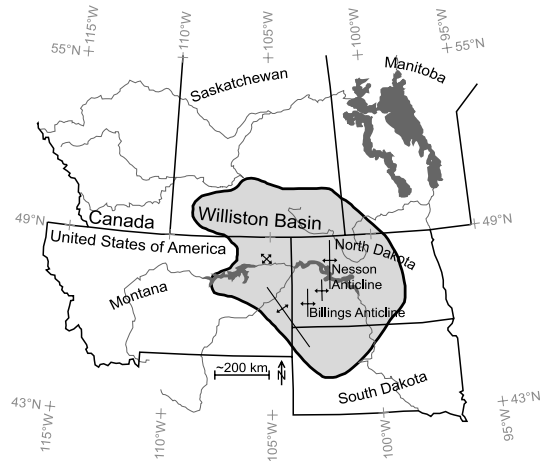
\includegraphics[scale=0.6]{bakken}
  }
  \caption{Расположение нефтегазоносного бассейна Уиллистон на границе США и Канады. Адаптировано с работы~\autocite{kuhn2012three}.}
  \label{fig:bakken}
\end{figure}

\begin{figure}[ht]
  \centerfloat{
    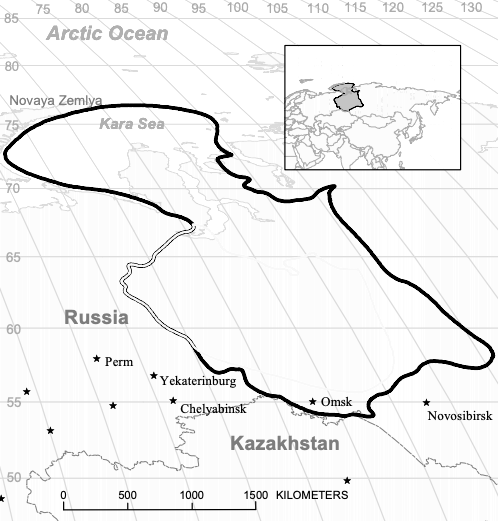
\includegraphics[scale=0.65]{bazhenov}
  }
  \caption{Расположение Баженовской свиты на территории Западной Сибири. Адаптировано с работы~\autocite{USGS}.}
  \label{fig:bazhenov}
\end{figure}

В то время как наличие естественных трещин является одной из ключевых характеристик в вопросах возможности добычи нефти и газа из низкопроницаемых пород, искусственные трещины, как правило образовавшиеся вследствие гидравлических разрывов (в англоязычной литературе устоялся термин OWHF или oil well hydraulic fracturing), лишь создают хоть сколько-нибудь проницаемую область (the SRV или Stimulated Reservoir Volume) в окрестности нефтедобывающей скважины~\autocite{warpinski2009stimulating}. Несмотря на бурное развитие технологий моделирования добычи нефти и газа из низкопроницаемых коллекторов в последнее двадцатилетие, известные математические модели не объясняют многие физические процессы в таких геологических породах. При непосредственной разработке таких резервуаров в среде проявляются различные нелинейные эффекты, нелинейные или не подчиняющиеся закону Дарси течения, а также так называемый Klinkenberg-эффект,~--- эффект прилипания/скольжения молекул газа (gas slip effect)  при течении в пористой среде. К числу перечисленных выше явлений также относят абсорбцию и десорбцию, сложное межмолекулярное взаимодействие (газ с водой, твердое тело с мелкими порами), трещинообразование. Вследствие этих нелинейных физических процессов и явлений, на сегодня в литературе имеет место быть лишь базовое представление о том, как движется нефть или газ в таких породах, и нет устоявшегося представления о том, как формируются и развиваются трещины в таких плотных неоднородных и неизотропных породах~\autocite{warpinski2009stimulating, wu2014generalized}.

Предлагаемая в данной работе модель двойной пористой среды с упругим трещиноватым скелетом дает физически качественное объяснение ряду физических процессов, связанных с аномально высоким пластовым давлением и трещинообразованием, и, как следствие, демонстрирует принципиальную возможность формирования подобной вышеописанной проницаемой области в окрестности скважины только благодаря аномально высокому пластовому давлению.

Давление в порах называется аномально высоким, если оно превышает гидростатический уровень. Аномально высокое пластовое давление, или АВПД (overpressure или abnormal pressure), является распространенным явлением в пластовых породах со сверхнизкой проницаемостью, таких как карбонаты, известняки и сланцы~\autocite{fertl1976abnormal, luo2002natural, melik1983, magara1978significance}. Выделяют несколько причин возникновения АВПД связанных с историей формирования залежи, термическим состоянием пласта, физико-химическими процессами, движением флюидов в земной коре. В частности, основным механизмом формирования АВПД в нефтематеринских породах является генерация флюида в условиях сверхнизкой проницаемости (созревание керогена в условиях низкой проницаемости). Аномально высокое пластовое давление достигает значений до 0.95 от горного давления~\autocite{li2012pore}, и может не только служить причиной разрушения стенок скважин~\autocite{melik1983, li2012pore}, но и способно поддерживать дебит нефти в низкопроницаемых коллекторах в отсутствие возможности применения традиционных методов поддержания пластового давления~\autocite{sonnenberg2009petroleum}. Кроме того, аномально высокое пластовое давление может приводить к развитию вторичных трещин в породе с низкой проницаемостью. Это явление, называемое автофлюидоразрыв или в англоязычной литературе как NHF (natural hydraulic fracturing), хорошо известно и обсуждается в связи с проблемой миграции флюидов~\autocite{secor1965role, engelder1990natural, luo2002natural}.

Первоначально концепция автофлюидоразрыва была развита в работах~\autocite{secor1965role} на основе подходов к моделированию традиционного гидроразрыва (OWHF). В~\autocite{secor1965role} рассматривается набор произвольно ориентированных трещин с непроницаемыми стенками на достаточно большом расстоянии друг от друга, чтобы исключить их взаимное влияние. В качестве критерия распространения трещин используется вариант энергетической теории Гриффитса. В дальнейшем эта модель была обобщена на случай пороупругой среды в предположении, что давление в трещинах в каждый момент времени равно поровому давлению в пространстве между трещинами~\autocite{engelder1990natural}. Указанные модели изначально сформулированы для описания развития трещиноватости в горных породах на геологических масштабах времени. При этом указывается, что автофлюидоразрыв играет важную роль в миграции флюидов. Например, если в силу определенных причин (например, созревание керогена в условиях низкой проницаемости) поровое давление в низкопроницаемом пласте, постепенно повышаясь, достигает критерия страгивания трещин (initiation), трещины начинают расти (propagation), что приводит к увеличению их объема, падению давления и, в результате, прекращению роста трещин (arrest). Процесс повторяется циклически. В работе~\autocite{luo2002natural} показано, что в сланцевых пластах при наличии АВПД возможно установление равновесия в окрестности критерия разрушения, когда генерируемый в нефтематеринской породе флюид отводится по системе трещин автофлюидоразрыва (зона I на рисунке~\ref{fig:NHF}).

В настоящей работе рассматривается ситуация, когда за длительный предшествующий период давление в матрице превысило гидростатический уровень, однако критерий разрушения еще не достигнут (например, зона II на рисунке~\ref{fig:NHF}). Считается, что разрушение в матрице может произойти при участии аномально высокого пластового давления в процессе технологических операций (например, бурение скважины, депрессия на забое скважины в процессе добычи и др.).

\begin{figure}[ht]
  \centerfloat{
    \includegraphics[scale=0.9]{NHF}
  }
  \caption{На следующем условном для данной работы рисунке (рисунок из~\autocite{luo2002natural}) по оси ординат сверху вниз отложено увеличение глубины, по абсцисс слева направо, - увеличение давления. Использованы следующие обозначения: [1]~--- аномально высокое пластовое давление, [2]~--- гидростатический уровень ($\rho g h$), [4]~--- условный критерий страгивания трещин, [3]~--- литостатический уровень.}
  \label{fig:NHF}
\end{figure}

Традиционно при описании движения флюидов в трещиновато-пористых коллекторах используют модель двойной пористости~\autocite{barenblatt1960basic, golf1986, wu2014generalized}. Такие трещиновато-пористые пласты состоят из блоков насыщенной пористой низкопроницаемой породы, называемой матрицей, разделенных магистральными трещинами, по которым двигается жидкость (см. рисунок~\ref{fig:barenblat}). При этом матрица осуществляет подпитку системы трещин. В основе семейства континуальных моделей среды с двойной пористостью, насыщенной одной жидкостью, лежит гипотеза суперпозиции трех континуумов (предполагается, что элементарный объем (REV или representative elementary volume), по которому проводится усреднение, много больше характерного расстояния между магистральными трещинами). Первый континуум образован частью жидкости, насыщающей матрицу, которая характеризуется низкой проницаемостью, но достаточно большой пористостью. Второй континуум образован жидкостью, заполняющей систему магистральных трещин, объемная доля которых мала по сравнению с пористостью матрицы. При этом проницаемость системы трещин предполагается достаточно высокой, чтобы обеспечить подвижность второго континуума. Третьим континуумом является твердый скелет, который может быть жестким, пороупругим или проявлять вязкие и пластические свойства. Стоит отметить, что, если блоки матрицы не изолированы, и проницаемость матрицы сравнима с проницаемостью трещин, модель двойной пористости часто называют моделью двойной проницаемости (и/или же моделью двойной проницаемости называют еще вследствие наличия разницы макроспкопических градиентов давлений между двумя подсистемами). Как правило, учет влияния аномально высокого пластового давления на производство нефти или газа в сланцевых породах сводится к учету зависимости проницаемости системы трещин в среде с двойной пористостью от давления~\autocite{thompson2010modeling} в связи с тем, что для движения флюидов в низкопроницаемых породах требуются значительные депрессии.

\begin{figure}[ht]
  \centerfloat{
    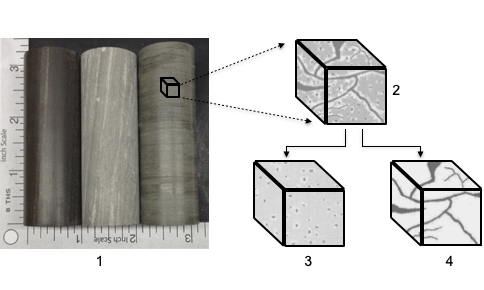
\includegraphics[scale=1]{comboimg}
  }
  \caption{Элементарный объем трещиноватой горной породы (2), состоящей из пор и проницаемых блоков (3), разделенных между собой системой трещин (4). (1)~--- три различных образца сланца из статьи~\autocite{ye2016fracture}. Адаптировано с работы~\autocite{abousleiman2005poromechanics}.}
  \label{fig:barenblat}
\end{figure}

В отличие от указанного подхода в данной работе развивается модель среды с двойной пористостью, матрица которой способна растрескиваться под действием аномально высокого пластового давления, тем самым увеличивая интенсивность массообмена между подсистемами матрицыи и трещины.

Развитие системы трещин, длина которых много меньше характерного размера элементарного объема, естественно моделировать методами теории повреждаемых сред (CDM~--- continuum damage mechanics)~\autocite{lemaitre2012course, murakami2012continuum}, в рамках которой коллектив микротрещин описывается осредненно с помощью специального параметра поврежденности. В настоящей работе для моделирования автофлюидоразрыва в матрице используется модель повреждаемости, аналогичная~\autocite{kondaurov2007, izvekov2009, izvekov2010}. Для простоты использован скалярный параметр поврежденности, что соответствует случайному распределению трещин по направлениям в пространстве. Критерий инициации начала развития повреждаемости в модели~\autocite{kondaurov2007, izvekov2009, izvekov2010} является своеобразным обобщением энергетического критерия Гриффитса на случай рассеянного разрушения хрупких сред. Предполагается, что возникающие микротрещины в матрице в первую очередь усиливают массообмен между матрицей и магистральными трещинами.



% {\progress}
% Этот раздел должен быть отдельным структурным элементом по
% ГОСТ, но он, как правило, включается в описание актуальности
% темы. Нужен он отдельным структурынм элемементом или нет ---
% смотрите другие диссертации вашего совета, скорее всего не нужен.

{\aim} данной работы является моделирование влияния аномально высокого пластового давления в двойной пористой среде с упругим трещиноватым скелетом.

Для~достижения поставленной цели необходимо было решить следующие {\tasks}:
\begin{enumerate}
  \item Разработать физическую модель, учитывающую аномально высокое пластовое давление в двойной пористой среде с упругим трещиноватым скелетом;
  \item Исследовать параметры модели, сделать численные оценки этих параметров;
  \item Провести численный расчет для рассматриваемой модели на примере задачи о производительности скважины.
\end{enumerate}


{\novelty}
\begin{enumerate}
  \item Учтено влияния аномально высокого пластового давления в двойной пористой среде, используя детерминистический параметр повреждаемости, таким образом матрица способна растрескиваться под действием аномально высокого пластового давления, - основное отличие от традиционных моделей двойной пористой среды;
  \item В отличие от работ концепции автофлюидоразрыва, в данной работе решается задача о производительности скважины, при этом рассматривается зона II на рисунке~\ref{fig:NHF}, когда за длительный предшествующий промежуток времени накопилось аномально высокое пластовое давление, но инициации развития трещин еще не было.
  \item Показаны закономерности работы скважины, в окрестности которой идут процессы разрушения за счет энергии накопленного аномально высокого пластового давления.
\end{enumerate}

%{\influence} \ldots

%{\methods} \ldots

%{\defpositions}
%\begin{enumerate}
%  \item Первое положение
%  \item Второе положение
%  \item Третье положение
%  \item Четвертое положение
%\end{enumerate}
%В папке Documents можно ознакомиться в решением совета из Томского ГУ
%в~файле \verb+Def_positions.pdf+, где обоснованно даются рекомендации
%по~формулировкам защищаемых положений.

%{\reliability} полученных результатов обеспечивается \ldots \ Результаты находятся в соответствии с результатами, %полученными другими авторами.


{\probation}
Основные результаты работы докладывались~на следующих конференциях:
\begin{enumerate}
  \item Международная конференция по геофизическим наукам (The EGU General Assembly), Вена, Австрия, 2019~\cite{eguconf}.
  \item Международная конференция по физике высоких температур и взаимодейтсвию материалов (XXXIV International Conference on Interaction of Intense Energy Fluxes with Matter), Эльбрус, Кабардино-Балкария, Россия, 2019~\cite{ivtanconf}.
  \item 61 научная конференция МФТИ, Долгопрудный, Россия, 2018~\cite{miptconf}.
\end{enumerate}

{\contribution} Автор принимал активное участие в обсуждении теоретических положений и алгоритма численного решения, а также в реализации алгоритма и интерпретации полученных результатов.

{\publications} Основные результаты по теме диссертации изложены в 1 научной статье,
каторая принята в печать журналом <<Физика Земли>>~\cite{fizzemli2020}.

% \ifnumequal{\value{bibliosel}}{0}
% {%%% Встроенная реализация с загрузкой файла через движок bibtex8. (При желании, внутри можно использовать обычные ссылки, наподобие `\cite{vakbib1,vakbib2}`).
%     {\publications} Основные результаты по теме диссертации изложены
%     в~XX~печатных изданиях,
%     X из которых изданы в журналах, рекомендованных ВАК,
%     X "--- в тезисах докладов.
% }%
% {%%% Реализация пакетом biblatex через движок biber
%     \begin{refsection}[bl-author]
%         % Это refsection=1.
%         % Процитированные здесь работы:
%         %  * подсчитываются, для автоматического составления фразы "Основные результаты ..."
%         %  * попадают в авторскую библиографию, при usefootcite==0 и стиле `\insertbiblioauthor` или `\insertbiblioauthorgrouped`
%         %  * нумеруются там в зависимости от порядка команд `\printbibliography` в этом разделе.
%         %  * при использовании `\insertbiblioauthorgrouped`, порядок команд `\printbibliography` в нём должен быть тем же (см. biblio/biblatex.tex)
%         %
%         % Невидимый библиографический список для подсчёта количества публикаций:
%         \printbibliography[heading=nobibheading, section=1, env=countauthorvak,          keyword=biblioauthorvak]%
%         \printbibliography[heading=nobibheading, section=1, env=countauthorwos,          keyword=biblioauthorwos]%
%         \printbibliography[heading=nobibheading, section=1, env=countauthorscopus,       keyword=biblioauthorscopus]%
%         \printbibliography[heading=nobibheading, section=1, env=countauthorconf,         keyword=biblioauthorconf]%
%         \printbibliography[heading=nobibheading, section=1, env=countauthorother,        keyword=biblioauthorother]%
%         \printbibliography[heading=nobibheading, section=1, env=countauthor,             keyword=biblioauthor]%
%         \printbibliography[heading=nobibheading, section=1, env=countauthorvakscopuswos, filter=vakscopuswos]%
%         \printbibliography[heading=nobibheading, section=1, env=countauthorscopuswos,    filter=scopuswos]%
%         %
%         \nocite{*}%
%         %
%         {\publications} Основные результаты по теме диссертации изложены в 1 печатном издании,
%         которое издано в журнале <<Физика Земли>> (Q2 по данным 2019 г.)~\cite{fizzemli2020}
%         % \ifnum \value{citeauthorconf}>0%
%             , 3 "--- в~тезисах докладов конференций.
%         % \else%
%             % .
%         % \fi
%     \end{refsection}%
%     \begin{refsection}[bl-author]
%         % Это refsection=2.
%         % Процитированные здесь работы:
%         %  * попадают в авторскую библиографию, при usefootcite==0 и стиле `\insertbiblioauthorimportant`.
%         %  * ни на что не влияют в противном случае
%         \nocite{vakbib2}%vak
%         \nocite{bib1}%other
%         \nocite{confbib1}%conf
%     \end{refsection}%
%         %
%         % Всё, что вне этих двух refsection, это refsection=0,
%         %  * для диссертации - это нормальные ссылки, попадающие в обычную библиографию
%         %  * для автореферата:
%         %     * при usefootcite==0, ссылка корректно сработает только для источника из `external.bib`. Для своих работ --- напечатает "[0]" (и даже Warning не вылезет).
%         %     * при usefootcite==1, ссылка сработает нормально. В авторской библиографии будут только процитированные в refsection=0 работы.
%         %
%         % Невидимый библиографический список для подсчёта количества внешних публикаций
%         % Используется, чтобы убрать приставку "А" у работ автора, если в автореферате нет
%         % цитирований внешних источников.
%         % Замедляет компиляцию
%     \ifsynopsis
%     \ifnumequal{\value{draft}}{0}{
%       %
%     }{}
%     \fi
%     \printbibliography[heading=nobibheading, section=0, env=countexternal,          keyword=biblioexternal]
% }
